\documentclass[tikz,border=10pt]{standalone}
\usepackage{tikz}
\usepackage{amsmath,amsfonts,graphicx,amsthm}

\begin{document}

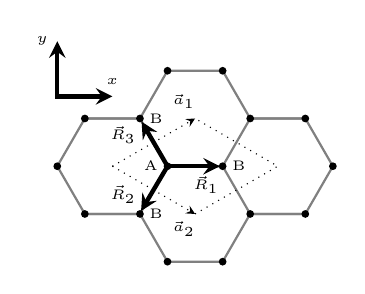
\begin{tikzpicture}[scale=0.7]
        %\draw[step=1cm,gray,very thin] (0,0) grid (9,4);
        \draw[ultra thick,black,stealth-stealth] (2,4) -- (2,3) -- (3,3);
        \node[below] at (3,3.5){\tiny $x$};
        \node[left] at (2,4){\tiny $y$};
        
        % y= 0 line
        \draw[thick, gray]  (2.5,0.8660254038) -- (3.5,0.8660254038) -- (4,0) -- (5,0) -- (5.5,0.8660254038) -- (6.5,0.8660254038);
        \draw[thick, gray] (2,1.732050808) -- (2.5,0.8660254038) -- (3.5,0.8660254038) -- (4,1.732050808) -- (5,1.732050808) -- (5.5,0.8660254038) -- (6.5,0.8660254038) -- (7,1.732050808);
        \draw[thick, gray] (2,1.732050808) -- (2.5,2.598076211) -- (3.5,2.598076211) -- (4,1.732050808) -- (5,1.732050808) -- (5.5,2.598076211) -- (6.5,2.598076211) -- (7,1.732050808);
        \fill[black]      (4,0)                   circle(2pt);
        \fill[black]    (5,0)                   circle(2pt);
        
        % Unit Cell Dotted
         \draw[black,dotted, -stealth] (3,1.732050808) -- (4.5,0.8660254038);
         \draw[ dotted, black] (4.5,0.8660254038) -- (6,1.732050808) -- (4.5,2.598076211);
        \node[below] at (4.3,0.9){\tiny $\Vec{a}_{2}$};
        \draw[black,dotted, -stealth] (3,1.732050808) -- (4.5,2.598076211);
        \node[above] at (4.3,2.6){\tiny $\Vec{a}_{1}$};
        % Position Vectors
        \node [left] at (4,1.732050808) {\tiny A};
        \node [right] at (5,1.732050808) {\tiny B};
        \node [right] at (3.5,0.8660254038) {\tiny B};
        \node [right] at (3.5,2.598076211) {\tiny B};
        \draw[ultra thick, black, -stealth] (4,1.732050808) -- (4.95,1.732050808);
        \node[below] at (4.7,1.732050808) {\tiny $\Vec{R}_{1}$};
        \draw[ultra thick, black, -stealth] (4,1.732050808) -- (3.52,0.92);
        \node[left] at (3.6,1.22) {\tiny $\Vec{R}_{2}$};
        \draw[ultra thick, black, -stealth] (4,1.732050808) -- (3.53,2.54);
        \node[left] at (3.6,2.3) {\tiny $\Vec{R}_{3}$};
        
        
        % Graphene Background Structure
        % y= 0.8660254038 line
        \fill[black]      (2.5,0.8660254038)      circle(2pt);
        \fill[black]    (3.5,0.8660254038)      circle(2pt);
        \fill[black]      (5.5,0.8660254038)      circle(2pt);
        \fill[black]    (6.5,0.8660254038)      circle(2pt);
        % y = 1.732050808 line
        \fill[black]      (2,1.732050808)         circle(2pt);
        \fill[black]      (4,1.732050808)         circle(2pt);
        \fill[black]    (5,1.732050808)         circle(2pt);
        \fill[black]      (7,1.732050808)         circle(2pt);
        \draw[thick, gray] (2.5,2.598076211) -- (3.5,2.598076211) -- (4,3.464101615) -- (5,3.464101615) -- (5.5,2.598076211) -- (6.5,2.598076211);
        % y= 2.598076211 line
        \fill[black]      (2.5,2.598076211)      circle(2pt);
        \fill[black]    (3.5,2.598076211)      circle(2pt);
        \fill[black]      (5.5,2.598076211)      circle(2pt);
        \fill[black]    (6.5,2.598076211)      circle(2pt);
        % y = 3.464101615 line
        \fill[black]      (4,3.464101615)         circle(2pt);
        \fill[black]    (5,3.464101615)         circle(2pt);
        \end{tikzpicture}
        \end{document}